\documentclass[tikz,border=2mm]{standalone}
\usepackage{amsmath}
\usepackage{amssymb}
\usepackage{tikz}
\usetikzlibrary{arrows.meta,positioning,fit,backgrounds,calc}

\definecolor{lightblue}{RGB}{173,216,230}
\definecolor{lightgreen}{RGB}{144,238,144}
\definecolor{lightyellow}{RGB}{255,250,205}
\definecolor{lightred}{RGB}{255,182,193}
\definecolor{lightgray}{RGB}{240,240,240}
\definecolor{alphablue}{RGB}{47,102,194}
\definecolor{betared}{RGB}{196,64,64}
\definecolor{edgegreen}{RGB}{42,135,58}
\definecolor{edgeorange}{RGB}{220,120,25}
\definecolor{edgepurple}{RGB}{135,55,150}

\begin{document}
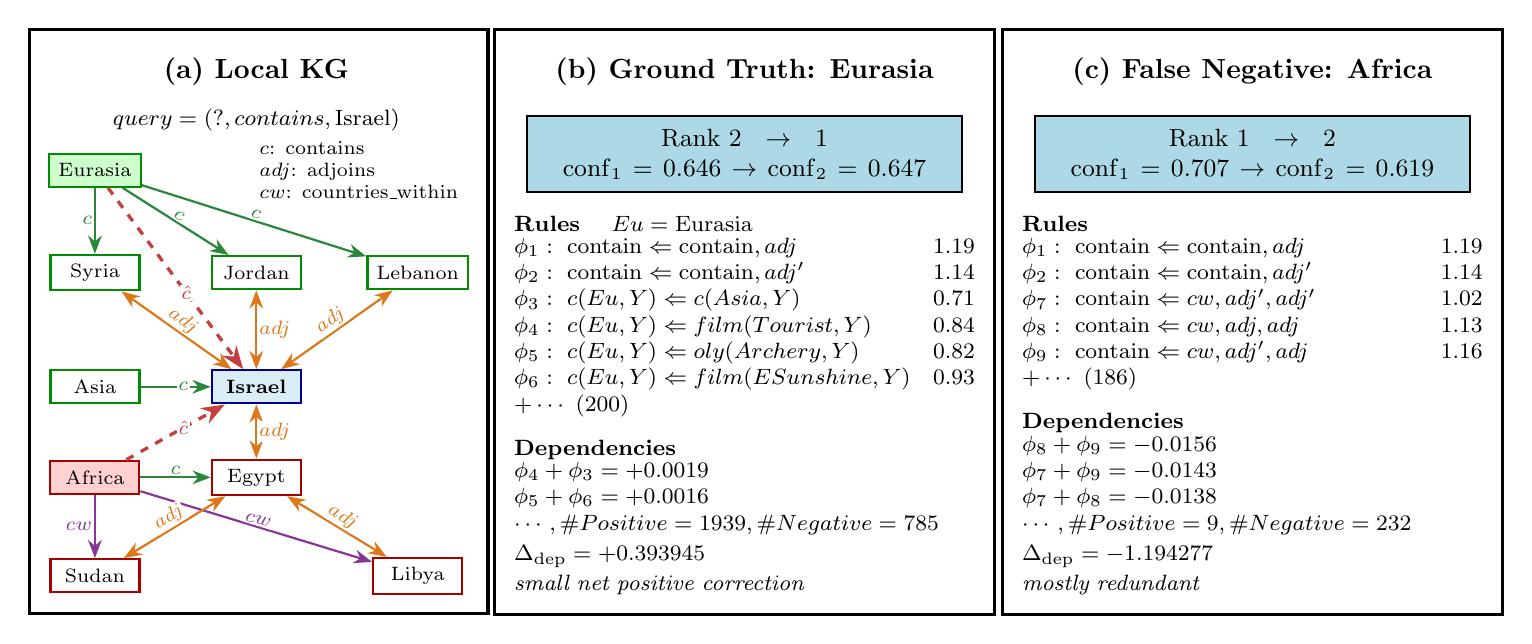
\begin{tikzpicture}[
    node distance=0.22cm,
    box/.style={rectangle, draw, thick, minimum width=2.8cm, minimum height=0.55cm, align=center, font=\small},
    title/.style={font=\bfseries\normalsize},
    formula/.style={font=\footnotesize, align=left},
    section/.style={rectangle, draw=black, very thick, inner sep=2.4mm},
    ent/.style={rectangle, draw, thick, minimum width=1.13cm, minimum height=0.42cm, align=center, font=\scriptsize},
    gt/.style={ent, fill=white, draw=green!55!black},
    cone/.style={ent, fill=white, draw=red!65!black},
    gtfocus/.style={gt, fill=green!20, line width=0.75pt},
    conefocus/.style={cone, fill=red!18, line width=0.75pt},
    qent/.style={ent, fill=lightblue!45, draw=blue!60!black, font=\scriptsize\bfseries},
    contains/.style={-Stealth, thick, edgegreen},
    countries/.style={-Stealth, thick, edgepurple},
    adjoins/.style={Stealth-Stealth, thick, edgeorange},
    pred/.style={-Stealth, very thick, dashed, betared},
    elab/.style={font=\scriptsize, fill=white, inner sep=0.6pt},
    legend/.style={font=\scriptsize, align=left}
]

% ============ (a) Local KG ============
\node[title] (title-a) at (0,0) {(a) Local KG};
\node[formula, below=0.05cm of title-a] (query) {$query=(?,contains,\mathrm{Israel})$};

\node[gtfocus] (eurasia) at (-2.05,-1.25) {Eurasia};
\node[gt] (syria)   at (-2.05,-2.55) {Syria};
\node[gt] (jordan)  at (0.00,-2.55) {Jordan};
\node[gt] (lebanon) at (2.05,-2.55) {Lebanon};
\node[gt] (asia)    at (-2.05,-4.00) {Asia};
\node[qent] (israel) at (0.00,-4.00) {Israel};
\node[conefocus] (africa) at (-2.05,-5.15) {Africa};
\node[cone] (egypt)  at (0.00,-5.15) {Egypt};
\node[cone] (sudan)  at (-2.05,-6.4) {Sudan};
\node[cone] (libya)  at (2.05,-6.4) {Libya};
\node[legend] (kg-legend) at (1.3,-1.25) {$c$: contains\\$adj$: adjoins\\$cw$: countries\_within};

\draw[contains] (asia) -- node[elab,right] {$c$} (israel);
\draw[contains] (eurasia) -- node[elab,left] {$c$} (syria);
\draw[contains] (eurasia) -- node[elab,above,sloped] {$c$} (jordan);
\draw[contains] (eurasia) -- node[elab,above,sloped] {$c$} (lebanon);
\draw[adjoins] (syria) -- node[elab,above,sloped] {$adj$} (israel);
\draw[adjoins] (jordan) -- node[elab,right] {$adj$} (israel);
\draw[adjoins] (lebanon) -- node[elab,above,sloped] {$adj$} (israel);
\draw[contains] (africa) -- node[elab,above] {$c$} (egypt);
\draw[countries] (africa) -- node[elab,left] {$cw$} (sudan);
\draw[countries] (africa) -- node[elab,above,sloped] {$cw$} (libya);
\draw[adjoins] (egypt) -- node[elab,right] {$adj$} (israel);
\draw[adjoins] (egypt) -- node[elab,above,sloped] {$adj$} (sudan);
\draw[adjoins] (egypt) -- node[elab,above,sloped] {$adj$} (libya);
\draw[pred] (eurasia) -- node[elab,pos=0.58] {$\hat c$} (israel);
\draw[pred] (africa) -- node[elab,pos=0.58] {$\hat c$} (israel);

\begin{scope}[on background layer]
\node[section, fit=(title-a)(query)(eurasia)(asia)(syria)(jordan)(lebanon)(israel)(africa)(egypt)(sudan)(libya)(kg-legend)] (sec-a) {};
\end{scope}

% ============ (b) GT ============
\node[title] (title-b) at (6.2,0) {(b) Ground Truth: Eurasia};

\node[box, fill=lightblue, below=0.25cm of title-b, text width=5.2cm, inner sep=1.6mm] (gt-score) {
    Rank $2\to1$ \\
    $\mathrm{conf}_1=0.646 \to \mathrm{conf}_2=0.647$
};

\node[formula, below=0.28cm of gt-score, text width=5.85cm, inner sep=0mm] (gt-rules) {
    \textbf{Rules} $\quad Eu=\mathrm{Eurasia}$\\[-0.5mm]
    $\phi_1:\ \mathrm{contain}\Leftarrow \mathrm{contain},adj$ \hfill $1.19$\\
    $\phi_2:\ \mathrm{contain}\Leftarrow \mathrm{contain},adj'$ \hfill $1.14$\\
    $\phi_3:\ c(Eu,Y)\Leftarrow c(Asia,Y)$ \hfill $0.71$\\
    $\phi_4:\ c(Eu,Y)\Leftarrow film(Tourist,Y)$ \hfill $0.84$\\
    $\phi_5:\ c(Eu,Y)\Leftarrow oly(Archery,Y)$ \hfill $0.82$\\
    $\phi_6:\ c(Eu,Y)\Leftarrow film(ESunshine,Y)$ \hfill $0.93$\\
    $+\cdots\ (200)$
};

\node[formula, below=0.28cm of gt-rules, text width=5.85cm, inner sep=0mm] (gt-dep) {
    \textbf{Dependencies}\\[-0.5mm]
    $\phi_4+\phi_3=+0.0019$\\
    $\phi_5+\phi_6=+0.0016$\\
    $\cdots, \#Positive=1939, \#Negative=785$\\[0.5mm]
    $\Delta_{\rm dep}=+0.393945$\\[0.5mm]
    \textit{small net positive correction}
};

\begin{scope}[on background layer]
\node[section, fit=(title-b)(gt-score)(gt-rules)(gt-dep), inner sep=2.4mm] (sec-b) {};
\end{scope}

% ============ (c) C1 ============
\node[title] (title-c) at (12.65,0) {(c) False Negative: Africa};

\node[box, fill=lightblue, below=0.25cm of title-c, text width=5.2cm, inner sep=1.6mm] (c1-score) {
    Rank $1\to2$ \\
    $\mathrm{conf}_1=0.707 \to \mathrm{conf}_2=0.619$
};

\node[formula, below=0.28cm of c1-score, text width=5.85cm, inner sep=0mm] (c1-rules) {
    \textbf{Rules}\\[-0.5mm]
    $\phi_1:\ \mathrm{contain}\Leftarrow \mathrm{contain},adj$ \hfill $1.19$\\
    $\phi_2:\ \mathrm{contain}\Leftarrow \mathrm{contain},adj'$ \hfill $1.14$\\
    $\phi_7:\ \mathrm{contain}\Leftarrow cw,adj',adj'$ \hfill $1.02$\\
    $\phi_8:\ \mathrm{contain}\Leftarrow cw,adj,adj$ \hfill $1.13$\\
    $\phi_9:\ \mathrm{contain}\Leftarrow cw,adj',adj$ \hfill $1.16$\\
    $+\cdots\ (186)$
};

\node[formula, below=0.28cm of c1-rules, text width=5.85cm, inner sep=0mm] (c1-dep) {
    \textbf{Dependencies}\\[-0.5mm]
    $\phi_8+\phi_9=-0.0156$\\
    $\phi_7+\phi_9=-0.0143$\\
    $\phi_7+\phi_8=-0.0138$\\
    $\cdots,\#Positive=9, \#Negative=232$\\[0.5mm]
    $\Delta_{\rm dep}=-1.194277$\\[0.5mm]
    \textit{mostly redundant}
};

\begin{scope}[on background layer]
\node[section, fit=(title-c)(c1-score)(c1-rules)(c1-dep), inner sep=2.4mm] (sec-c) {};
\end{scope}

\end{tikzpicture}
\end{document}